%\documentclass[notheorems]{beamer}
%\documentclass[handout]{beamer}
%\documentclass[handout,notes=show]{beamer}

\usetheme{metropolis}
%\usecolortheme{dolphin}
% No navigation bars
\beamertemplatenavigationsymbolsempty

\graphicspath{{img/}}
\usepackage{amsmath, amssymb, amsfonts, tikz}
\usepackage[utf8x]{inputenc}
\usepackage[T1]{fontenc}
\usepackage[english]{babel}
\usepackage{tabularx}
\usepackage{mathtools}
\usepackage{xmpmulti}
\usepackage{color}
\definecolor{keywordcolor}{rgb}{0.7, 0.1, 0.1}   % red
\definecolor{commentcolor}{rgb}{0.4, 0.4, 0.4}   % grey
\definecolor{symbolcolor}{rgb}{0.0, 0.1, 0.6}    % blue
\definecolor{sortcolor}{rgb}{0.1, 0.5, 0.1}      % green

\usepackage{amsthm}
\theoremstyle{plain}
\newtheorem{theorem}{Theorem}[section]
\newtheorem{corollary}[theorem]{Corollary}
\newtheorem{lemma}[theorem]{Lemma}
\newtheorem{algorithm}[theorem]{Algorithm}
\newtheorem{proposition}[theorem]{Proposition}
\newtheorem{claim}[theorem]{Claim}
\newtheorem{fact}[theorem]{Fact}
\newtheorem{conjecture}[theorem]{Conjecture}
%% Definition-like environments, normal text
%% Numbering is in sync with theorems, etc
\theoremstyle{definition}
\newtheorem{definition}[theorem]{Definition}
\newtheorem{problem}[theorem]{Problem}
%% Remark-like environments, normal text
%% Numbering is in sync with theorems, etc
\theoremstyle{definition}
\newtheorem{remark}[theorem]{Remark}
\newtheorem{observation}[theorem]{Observation}
%% Example-like environments, normal text
%% Numbering is in sync with theorems, etc
\theoremstyle{definition}
\newtheorem{example}[theorem]{Example}
\newtheorem{question}[theorem]{Question}
\newcommand{\terminology}[1]{\textbf{#1}}

\newcommand{\NN}{\mathbf{N}}
\newcommand{\ZZ}{\mathbf{Z}}
\newcommand{\QQ}{\mathbf Q}
\newcommand{\CC}{\mathbf C}
\newcommand{\RR}{\mathbf R}
\newcommand{\FF}{\mathbf F}
\newcommand{\lt}{<}
\newcommand{\gt}{>}
\newcommand{\amp}{&}
\newcommand{\diff}{\mathop{}\!\mathrm{d}}
\newcommand{\ints}{\mathcal{O}}
\newcommand{\ideal}[1]{\mathfrak{#1}}
\usepackage{mathrsfs}\usepackage{cancel}
\newcommand{\Gal}[2]{\operatorname{Gal}(#1/#2)}
\newcommand{\absgal}[1]{\operatorname{Gal}(\overline{#1}/#1)}
\DeclareMathOperator{\USp}{USp}
\DeclareMathOperator{\Spec}{Spec}

\newcommand{\sheaf}[1]{\operatorname{\mathcal{#1}}}
\newcommand{\inv}{^{-1}}
\DeclareMathOperator{\norm}{Nm}
\DeclareMathOperator{\ord}{ord}
\DeclareMathOperator{\divisor}{div}
\DeclareMathOperator{\PP}{\mathbf{P}}
\DeclareMathOperator{\Hom}{Hom}
\DeclareMathOperator{\Mat}{Mat}
\DeclareMathOperator{\End}{End}

\newcommand{\lb}{[}
\newcommand{\rb}{]}


\usepackage{listings}
\def\lstlanguagefiles{tex/lstlean.tex}

\lstset{language=lean}


\author{Alex J. Best}
\date{BU Math Retreat 2019}
\title{Something to Lean on; fun with interactive theorem provers}

\begin{document}

\begin{frame}
  \titlepage

  \note[item]{Thank the audience for being awake.}
\end{frame}

%\begin{frame}
%\frametitle{Table of Contents}
%\tableofcontents[currentsection]
%\end{frame}

\begin{frame}{The problem}
    Mathematicians make mistakes.

    \pause

    Sometimes they publish these mistakes.

    \pause

    Sometimes nobody notices.

    \pause

    At least for a while...
    \note{like a living organism mathematics notices and fixes itself eventually
    (this is harder for a false proof of a true statement!).
    }

    \pause
    However this uncertainty takes up time and energy, what if referees only needed to judge the importance, novelity and quality of exposition, not check the arguments.

\end{frame}

\begin{frame}{What is proof}\pause
    On an abstract level proof is a rigid mathematical concept.\pause

    In reality it is a social construct.\pause

    \begin{quotation}
        This story got me scared. Starting from 1993 multiple groups of mathematicians
        studied the “Cohomological Theory” paper at seminars and used it in their work
        and none of them noticed the mistake.

        And it clearly was not an accident. A technical argument by a trusted author, which is hard to check and looks similar to arguments known to be correct, is hardly ever checked in detail.

        --- Vladimir Voevodsky
    \end{quotation}

\end{frame}

\begin{frame}{Some examples: Grunwald(-Wang) and K-theory}

    \begin{quotation}
        Some days later I was with Artin in his office when Wang appeared. He said he had a counterexample to a lemma which had been used in the proof. An hour or two later, he produced a counterexample to the theorem itself... Of course he [Artin] was astonished, as were all of us students, that a famous theorem with two published proofs, one of which we had all heard in the seminar without our noticing anything, could be wrong.

        --- Tate
    \end{quotation}\pause

    \note{The problem: 2, the cursed prime. This is often an edge case.}

    \begin{quotation}
        The groundbreaking 1986 paper “Algebraic Cycles and Higher K-theory” by Spencer Bloch was soon after publication found by Andrei Suslin to contain a mistake in the proof of Lemma 1.1. The proof could not be fixed.

        --- Voevodsky
    \end{quotation}

\end{frame}

\begin{frame}{The solution}
    Work at an extremely high level of rigour, with every statement logical step spelled out in extreme detail and checked by multiple independent people.\pause

    \begin{problem}
        This is really boring!
    \end{problem}
    \pause

    \begin{quotation}
        But to do the work at the level of rigor and precision I felt was necessary would take an enormous amount of effort and would produce a text that would be very difficult to read. And who would ensure that I did not forget something and did not make a mistake, if even the mistakes in much more simple arguments take years to uncover?

        --- Voevodsky
    \end{quotation}


\end{frame}

\begin{frame}{The solution: Take 2}
    What if computers could do the boring work for us?\pause

    Computers are:
    \begin{itemize}
        \item Capable of checking basic logical statements,\pause
        \item Fast,\pause
        \item Never complain.
    \end{itemize}
\end{frame}

\begin{frame}{The new problem}
    How do you describe the steps of a proof to a computer with as little pain as possible? \pause
    Often mathematicians leave unsaid many steps which are intuitive or easily supplied. \note{(this is one place mistakes enter)}\pause

    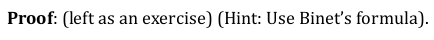
\includegraphics[height=2em]{pf-exercise.png}\pause

    
\includegraphics[height=1.5em]{beweis-klar.png}\pause

    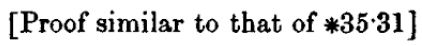
\includegraphics[height=1.5em]{pf-similar.png}\pause

    
\includegraphics[height=2em]{pf-obvious.png}\pause

    
\includegraphics[height=1.5em]{pf-remember.png}\pause

    
\includegraphics[height=1.1em]{pf-easy-induct.png}\pause

    The computer will probably not understand these, but in order to stay sane we must strike a balance between detail and verbosity.\note{ Teach the computer to work off as little as possible.}
\end{frame}

\begin{frame}{Enter Lean}
    The idea of trying this sort of thing has been around for a while. \pause

    But only within the last few years has it begun to seem more feasible for an average mathematician to do this. Tools have gotten better, slowly this idea has gained traction.\pause

    Recently an interactive proof assistant called Lean has been under heavy development. And I've been playing with it.

    Let me show you some lean code:
\end{frame}

\begin{frame}[fragile]
\begin{lstlisting}
lemma fact_rec (n : ℕ) :
factorial (n + 1) = factorial n * (n+1) :=
begin
-- write out the definition of factorial
unfold factorial,
-- remember {1,...,n+1} = {1,...,n} ∪ {n+1}
rewrite list.range'_concat 1 n,
-- the product of two sequences joined together is just the product of the products of each sequence
rewrite list.prod_append,
-- I'm bored already are we done here?
simp,
-- YES!
end
\end{lstlisting}\pause
We can replace all of the above with: \lstinline{by unfold factorial; simp [list.range'_concat, list.prod_append]}
\note{ Lean will figure out when and how to apply the lemmas.}

\end{frame}

\begin{frame}{(not so?) Live demo!}
    \multiinclude[<+->][format=png, graphics={width=\textwidth}]{fact}
\end{frame}

\begin{frame}{But can it do research?}
    Research level mathematics requires a vast body of knowledge to even think about.
    \pause

    As humans we forget this and also gloss over things we (think we) know well.
    \pause

    For instance one can forget what a Dedekind cut is, or Peano arithmetic and still think about real and natural numbers without an issue.
    Our intuition allows us to abstract these concepts so far away that we don't have to work from the ground up when approaching a problem.

\end{frame}


\begin{frame}{Perfectoids}
    Peter Scholze won a Fields medal in 2018 for ``transforming arithmetic algebraic geometry over $p$-adic fields through his introduction of perfectoid spaces, with application to Galois representations, and for the development of new cohomology theories.''
    \pause
    Within the past 10 years in number theory, this one definition above all others has revolutionised the way (some) people think.
    \pause
    The definition is highly nontrivial, an unusual geometric object created from an extremely non-Noetherian ring.
    \pause

    \emph{Last week} Kevin Buzzard, Johan Commelin, Patrick Massot  (and others)  completed a long term project to define a perfectoid space formally in Lean.
\end{frame}

\begin{frame}{Perfectoids}
    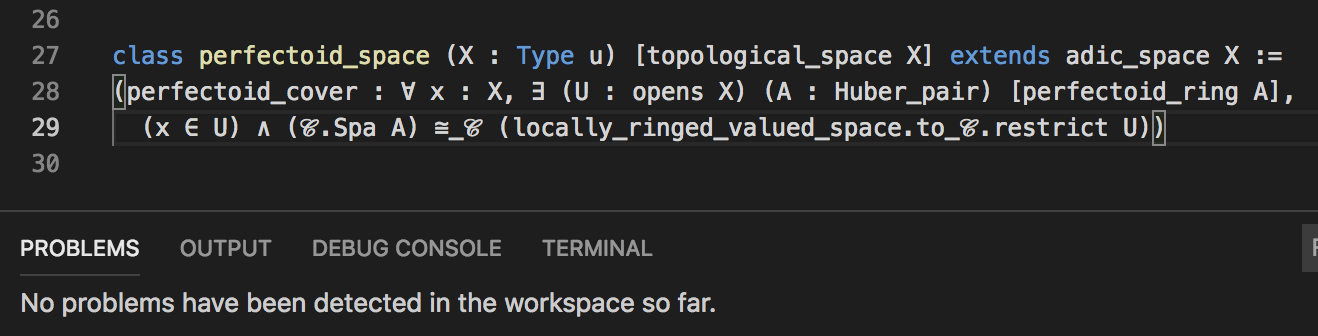
\includegraphics[width=\textwidth]{perfectoid.png}
    Lean has accepted the chain of definitions that lead to this are all valid, topological spaces, sheaves, valuations, adic spaces, perfectoid rings,...
    \pause

    It is difficult to estimate the amount of human effort expended to achieve this. \pause
    Their work relies on that of many others who are building \texttt{mathlib}, a general purpose library of mathematics from the ground up. \pause

    However, I would guess it compares favourably to the length of time needed to teach a human with zero mathematical background the same definition.
\end{frame}

\begin{frame}{A call to arms}
    I want to learn more about this!\pause

    Learning is better with others, the online lean community is great, (I posted and asked them to roast me and all they gave me was helpful tips), but nothing beats in person discussion.\pause

    If you think this sounds fun and/or interesting let me know, I'd love to organise a casual semi-regular meetup, to play with this together and collaborate!
\end{frame}

\end{document}
